\documentclass{article}
\usepackage[utf8]{inputenc}

% Preamble
\usepackage{amsmath}
\usepackage[margin=3cm, top=2cm, bottom=2cm]{geometry}
\usepackage{parskip}
   \setlength{\parindent}{0pt} % No automatic indent
\usepackage{setspace}
   \onehalfspacing
\usepackage{graphicx}
\usepackage{enumitem} % Lists
\usepackage{tabularx} % Tables
\usepackage{amssymb}  % For real numbers
\usepackage{dsfont}   % Indicator function (mathds{1})
%\usepackage[backend=bibtex]{biblatex}
\usepackage[round]{natbib}
\bibliographystyle{plainnat}
%\bibliography{bibliography}
\usepackage{placeins}
\usepackage{caption}

\usepackage{etoolbox}
\usepackage{float}  % Figure H placement
\patchcmd{\thebibliography}{\chapter*}{\section*}{}{} % Bibliography in same page
\usepackage{url}    % URL modes
%\decimalpoint % Point instead of comma for decimal places
\usepackage{hyperref}
%\usepackage{caption}
%\usepackage{subcaption}
\usepackage{wrapfig}
\usepackage[usenames, dvipsnames]{color}


%\usepackage{xcolor}
\usepackage[normalem]{ulem}
\useunder{\uline}{\ulined}{}%
\DeclareUrlCommand{\bulurl}{\def\UrlFont{\ttfamily\color{blue}\ulined}}


\begin{document}


\title{\vspace{-1.2cm}Text Mining the Sentiments Behind the Grammys}
\author{Gian Carlo Di-Luvi \\
{\normalsize Business Analytics Coordinator at Pfizer Inc.} \\
{\normalsize E-mail address: \href{mailto:giancarlo.diluvi@pfizer.com}{GianCarlo.Diluvi@pfizer.com}}}
\date{}

\maketitle


Music permeates our life as one of the most important forms of human expression. From our everyday activities to the most important moments in life, music is a part of it all. Like other art forms, music is a reflection of the world's overall problematics at any given time. There have naturally been many attempts to quantify music, and particularly song lyrics, in one way or another. In this paper, I use text mining and sentiment analysis to look at statistical aspects of lyrics of popular songs from 1960 onwards.

%Moreover, the entertainment industry is one of the biggest in the world, accounting for \hyperref[https://www.statista.com/statistics/237749/value-of-the-global-entertainment-and-media-market/]{more than \$1.5 trillion USD in 2015}. \\


%Of the many aspects of music, lyrics are of particular relevance because most contemporary artists impose their intended message within them. Thus, it is possible to draw meaningful conclusions of a song by analyzing its lyrics.  \\







\section*{Quantifying music}


The importance of music is such that a large number of awards are given on an almost constant basis to artists, producers, composers and all people involved in the music-making process. Their importance is that they highlight and recognize musicians that left a deep impact on the industry and, hence, on the world. This way, if one seeks to objectively study music, then musical awards may serve as a starting point. \\

As time passes, not only do bigger amounts of data become easier to access, but also in much more different forms. As such, it is of interest to develop techniques that allow us to analyze this ever-growing data heterogeneity. \textit{Text mining} is but one such set of techniques, whose purpose is to process, transform and study information in the form of text so that statistical conclusions can be derived from it. \\

%Text mining techniques can be applied to texts from different origins, such as political speeches, novels or, yes, song lyrics. With it, different texts can be objectively compared. \\

For this analysis, and with the help of the \texttt{geniusR} package in \textsf{R} (Parry, 2018), I obtained from \href{https://genius.com/}{\bulurl{Genius}} the lyrics (in English) of all the songs of each album that won the Grammy Award for Album of the Year from 1960 to date. The Grammy Awards, given every year to outstanding musicians, are arguably one of the most famous and prestigious musical awards. Grammy Awards are given for different categories, such as Record of the Year, Song of the Year, Best New Artist and Album of the Year. I chose the last one because it is awarded based on the quality of the album as a whole, and not on the merit of individual songs. It should be mentioned that 10 of these 58 albums' song lyrics were not available in Genius; those cases were simply omitted from the analysis. \\






%\begin{wrapfigure}{l}{0.6\textwidth}
%    \centering
%    \includegraphics[width=0.55\textwidth]{graph_common_words.png}
%    \caption{The ten most common words of the songs of all the albums that won the Grammy Award for Album of the Year are shown, along with the number of times they appear.}
%    \label{fig:common_words}
%\end{wrapfigure}


After joining the lyrics of the 668 songs in a single dataset, it is possible to obtain some interesting descriptive statistics. For instance, the average number of songs by album throughout time is roughly 14, with the 80s having a low 12.2 and the 2000s having the largest one at almost 16 (mainly due to Outkast's 2003 \textit{Speakerboxxx/The Love Below}, which contains an outstanding 40 songs.) \\

\newpage

There are exactly 160,206 words in total, averaging almost 240 by song. The 60s are by far the decade with the lowest average words by song, with 158, versus the much higher 295 in the past decade. Figure \ref{fig:common_words} shows the ten most common words in all those songs, without taking into account the usual English stop words such as `the', `of', `to', etc. 


\begin{figure}[h]
    \centering
    \includegraphics[scale=0.45]{Plots/graph_common_words.png}
    \caption{The ten most common words of the songs of all the albums that won the Grammy Award for Album of the Year are shown, along with the number of times they appear.}
    \label{fig:common_words}
\end{figure}



Amusingly, although perhaps not surprisingly, `love' is the most common word across all songs. Moreover, this is also true if one looks at each individual decade, as can be seen in Figure \ref{fig:common_words_decade}. This last Figure also shows that `baby' has been the second most popular word for the past three decades.


% na: Paul Simon's Diamond on the Soles of her Shows (unreleased version)
% ey: Taylor Swift's Wonderland
% la: The Boxer and Another Star
% ih: Homeless (Ft. Joseph Shabalala & Ladysmith Black Mambazo)

\begin{figure}[h]
    \centering
    \includegraphics[scale=0.6]{Plots/graph_common_words_decade_v2.png}
    \caption{The ten most common words of the songs of all the albums that won the Grammy Award for Album of the Year are shown, along with the number of times they appear in the $x$-axis, but now by decade.}
    \label{fig:common_words_decade}
\end{figure}





%\FloatBarrier
\section*{The sentiments of sentimentality}


Just by looking at the most common words by decade, it is possible to try to guess which decades were, say, happier than others. For example, `lonely' and `bad' (words with a negative tone) were very common words in the 60s, whereas `baby', `heart', `day' and `life' (words with a more positive tone) were more common in the 90s. This may lead us to hypothesize that the 90s had a lighter mood than the 60s. \\


The reasoning behind that example is the basis for \textit{sentiment analysis}, a series of techniques that help quantify emotions or affective states. Human writing is necessarily loaded of emotional intent in its words, and part of successful reading is the correct interpretation of those sentiments. Sentiment analysis aims to reproduce this mental process programmatically, using objective methods (without forgetting that, in the end, what is being studied is subjective by nature.) \\


%\newpage

There exist a variety of ways of doing this. The most popular ones rely on assigning sentiments to individual words, and then obtaining the net sentiment of a text by adding up the sentiments of the words that make it up. These so-called vocabulary lexicons contain a large number of English words with their respective sentiment (or sentiments) and are usually obtained and verified by crowdsourcing or even by hand. \\


\begin{wrapfigure}{l}{0.55\textwidth}
    \centering
    \includegraphics[width=0.5\textwidth]{Plots/graph_annual_sentiment.png}
    \caption{The net sentiment scores by album are shown, using color to differentiate between decades. Missing values correspond to the 10 albums whose song lyrics were not available in Genius.}
    \label{fig:annual_sentiment}
\end{wrapfigure}


For this analysis I used the \cite{Liu_sentiments} lexicon, which categorizes words as either `positive' or `negative' in a binary fashion. A `positive' and a `negative' score are computed by counting the number of words within each category, and the net sentiment is obtained by subtracting the latter from the former. Liu's lexicon can be found in the \texttt{sentiments} data set from the \texttt{tidytext} \textsf{R} package \citep{text_mining_r}. \\



I applied this lexicon to every song to generate a net sentiment score by album, which is shown on Figure \ref{fig:annual_sentiment}. From this graph we can see that the two albums with the greatest net sentiment belong to the 90s: Natalie Cole's 1992 \textit{Unforgettable... with Love} and Celine Dion's 1997 \textit{Falling into You}. Moreover, the 90s are the only decade in which no album has a negative net sentiment score. The 2010s are also an interesting decade in that they have the album with the third highest net sentiment (Bruno Mars' 2018 \textit{24K Magic}), and also the one with the lowest one (Mumford \& Sons' 2013 \textit{Babel}.)

%\begin{figure}[h]
%    \centering
%    \includegraphics[scale=0.45]{graph_annual_sentiment.png}
%    \caption{The net sentiment scores by album are shown, using color to differentiate between decades.}
%    \label{fig:annual_sentiment}
%\end{figure}

%\newpage

Notoriously, the 90s do appear to have albums with a greater net sentiment than the 60s', evidence that appears to favor our previous hypothesis (although the 60s do not seem to be a decade with particularly low net sentiments, as do the 00s, e.g.) In order to further confirm this, I obtained the average net sentiment of all the albums by decade, which is shown in Figure \ref{fig:decade_sentiment}. \\

By doing this it becomes evident that the 90s were the decade with the highest average net sentiment, with the 60s coming in second. Interestingly, the other decades' average net sentiment seems to vary around the same value of 30, making the 60s and 90s' much higher than average with net sentiments of 44 and 60, respectively.


\begin{figure}[h]
    \centering
    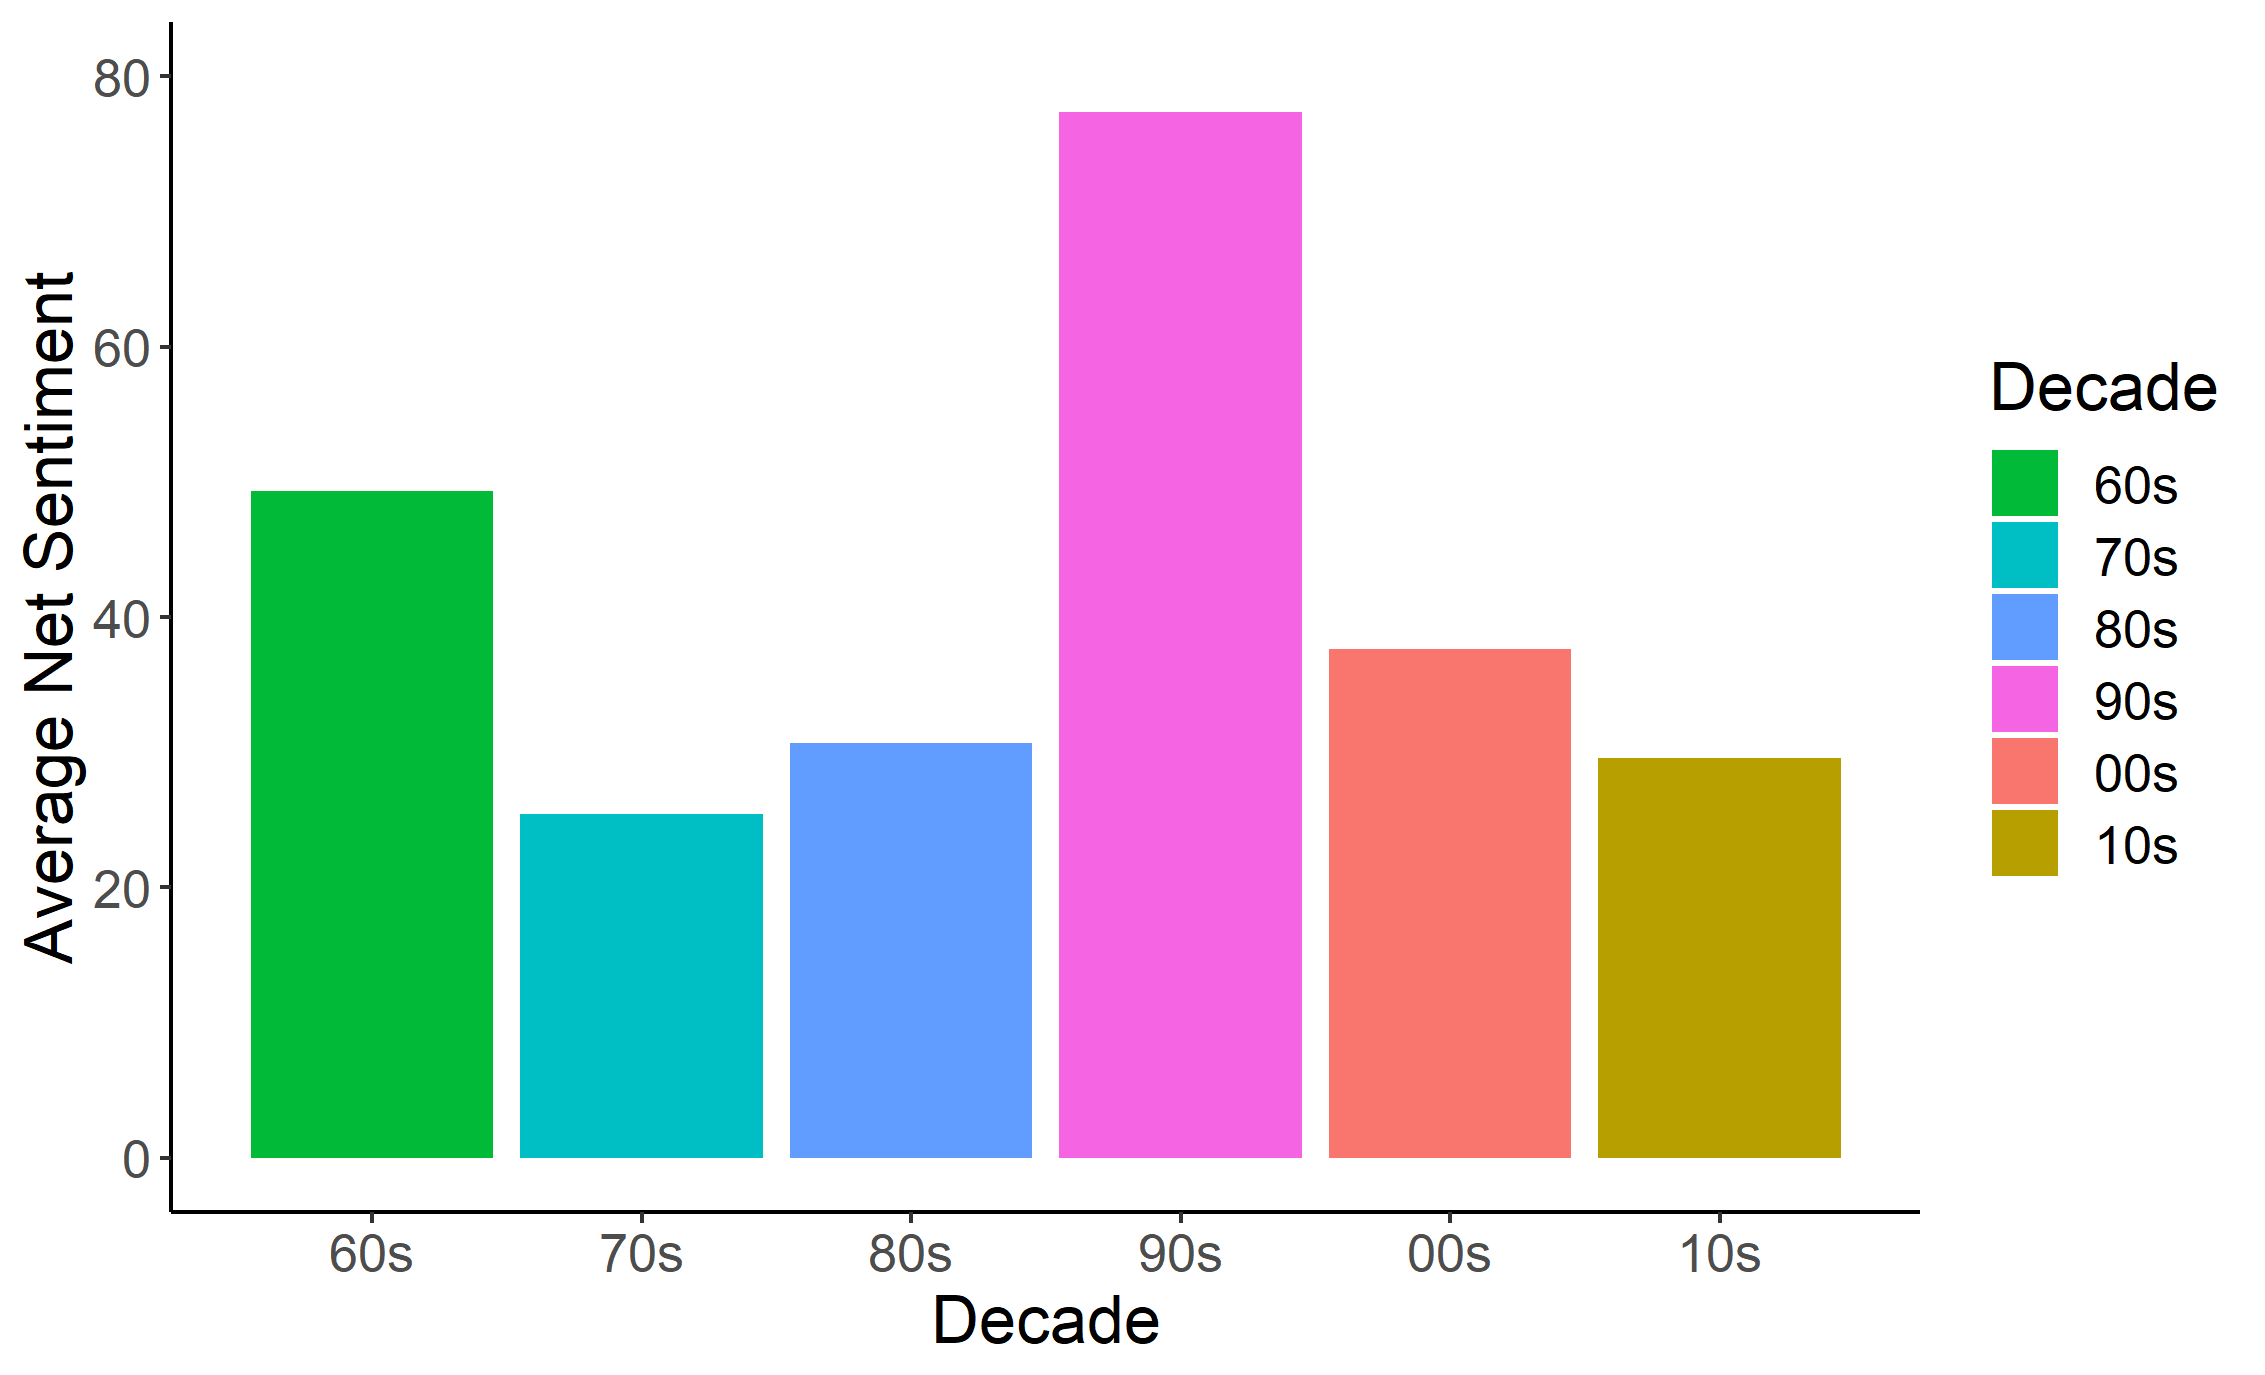
\includegraphics[scale=0.45]{Plots/graph_decade_mean_sentiment.png}
    \caption{The average net sentiment album scores by decade are shown.}
    \label{fig:decade_sentiment}
\end{figure}


\FloatBarrier



\section*{Betting on the Grammys}


Having obtained the net sentiment of every album that has won the Grammy Award for Album of the Year, it is possible to compute descriptive statistics of interest. For example, the average net sentiment of these albums is roughly 37, and half of them are between -39 and 123. In order to better quantify this, I obtained their \textit{probability density function} (pdf). This was done by a process called \textit{kernel smoothing}, which is very commonly used to estimate real-valued functions. I then used this information to estimate the probability of an album winning the Grammy Award based on its net sentiment as follows. \\


%\begin{figure}
%    \centering
%    \includegraphics[scale = 0.3]{graph_sentiment_density.png}
%    \caption{Plot of the probability density function of the net sentiment of albums that have won the Grammy Award for Album of the Year.}
%    \label{fig:density}
%\end{figure}


%\begin{figure}[h]
%\centering
%\begin{subfigure}{0.45\textwidth}
%  \centering
%  \includegraphics[width=0.45\linewidth]{graph_sentiment_density.png}
%  \caption{Plot of the probability density function of the net sentiment of albums that have won the Grammy Award for Album of the Year.}
%  \label{fig:density}
%\end{subfigure}%
%\begin{subfigure}{0.45\textwidth}
%  \centering
%  \includegraphics[width=0.45\linewidth]{graph_sentiment_posterior_density.png}
%  \caption{Plot of the probability density function of being awarded a Grammy given the sentiment, which is plotted in the $x$-axis.}
%  \label{fig:posterior_density}
%\end{subfigure}
%\caption{}
%\label{fig:densities}
%\end{figure}





The importance of knowing (at least approximately) the pdf is that it allows us to compute probabilities regarding the net sentiment of an album, given that it won the Grammy Award. That is, and using colors to better identify the factors under study, I obtained {\color{RoyalBlue} $P(\text{sentiment} \, | \, \text{Grammy})$}. Now imagine we could change the order and be able to compute probabilities of an album winning the Grammy Award, given its sentiment, {\color{Salmon} $P( \text{Grammy} \, | \, \text{sentiment} )$}. This can be done with the formula
\begin{equation*}
    {\color{Salmon} P( \text{Grammy} \, | \, \text{sentiment} )} = \frac{ {\color{RoyalBlue}  P(\text{sentiment} \, | \, \text{Grammy})} \times {\color{ForestGreen} P( \text{Grammy} )} }{ {\color{Brown} P( \text{sentiment} )} },
\end{equation*}
which is also known as \textit{Bayes' Theorem}. To summarise, by obtaining the net sentiments of albums that have won the Grammy Award we can effectively describe their behaviour, from a probabilistic point of view. Bayes' Theorem allows us to use this information to compute the probability of an album winning the Grammy Award, given that we know its net sentiment. Succinctly, we know {\color{RoyalBlue}blue} and want to obtain {\color{Salmon}red} = {\color{RoyalBlue}blue} $\times$ {\color{ForestGreen}green} / {\color{Brown}brown}. \\

%\begin{figure}[h]
%    \centering
%    \includegraphics[scale = 0.3]{graph_sentiment_posterior_density.png}
%    \caption{Plot of the probability density function of being awarded a Grammy given the sentiment, which is plotted in the $x$-axis.}
%    \label{fig:posterior_density}
%\end{figure}


%\begin{wrapfigure}{l}{0.55\textwidth}
%    \centering
%    \includegraphics[width=0.5\textwidth]{graph_densities_together.png}
%    \caption{The three probability density functions computed are shown.}
%    \label{fig:densities}
%\end{wrapfigure}


The only caveat is that we know neither {\color{ForestGreen} $P(\text{Grammy})$} nor {\color{Brown} $P(\text{sentiment})$}. The former refers to our initial beliefs regarding an album's probabilities of winning the Grammy Award. I decided to pick {\color{ForestGreen} $P(\text{Grammy})$} so that it reflected no initial beliefs on the matter. This is to say that, prior to obtaining any information, there is no net sentiment that entails a greater chance of winning the Award. \\

%This is commonly done when one does not want that probability to heavily influence the rest of the analysis. \\

I then used a Markov chain Monte Carlo (MCMC) method to obtain values of {\color{Salmon} $P( \text{Grammy} \, | \, \text{sentiment} )$}. These methods became popular in the 90s and are commonly used to solve problems in which values from a pdf are needed but can not be easily obtained. It was not necessary to estimate {\color{Brown} $P(\text{sentiment})$} because it is only a normalizing constant, and those have no effect when using this MCMC method, so that they can be omitted. \\

Figure \ref{fig:densities} shows the resulting pdf of {\color{Salmon} $P( \text{Grammy} \, | \, \text{sentiment} )$}. With it, we can now estimate, given an album's net sentiment, its probability of winning the Grammy Award for Album of the Year. \\ 


\begin{figure}[h]
    \centering
    \includegraphics[scale=0.6]{Plots/graph_posterior_density.png}
    \caption{The pdf of {\color{Salmon} $P( \text{Grammy} \, | \, \text{sentiment} )$} is shown.}
    \label{fig:densities}
\end{figure}{}

\newpage

\begin{wrapfigure}{l}{0.4\textwidth}
    \centering
    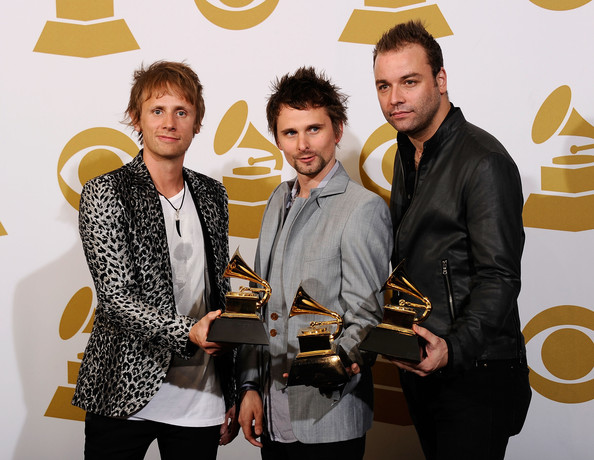
\includegraphics[width=0.37\textwidth]{Plots/MuseGrammys.jpg}
    \caption*{Muse pose in the press room at The 53rd Grammy Awards after winning the Grammy Award for Best Rock Album for \textit{The Resistance} on February 2011. Source: \href{http://www.zimbio.com/photos/Dominic+Howard/Matt+Bellamy/53rd+Annual+GRAMMY+Awards+Press+Room/Olbz7K-nebK}{\bulurl{Zimbio}}.}
\end{wrapfigure}

As an example, I decided to estimate the probability that my favorite band, Muse, wins the next Grammy Award for Album of the Year. Muse are an English rock band formed in 1994, and they have already won two Grammy Awards for Best Rock Album (in 2011 for \textit{The Resistance} and again in 2016 for their latest work, \textit{Drones}.) Now, Muse are expected to release a new album this year, with two singles, ``Dig Down'' and ``Thought Contagion'', already out. I obtained these songs' lyrics and computed their net sentiment, obtaining 2 and -5, respectively. Assuming that their new album will have a net sentiment between these values, I calculated their probability of winning the Grammy by numerically approximating the area below the {\color{Salmon}red} pdf of Figure \ref{fig:densities} between -5 and 2. I got an estimate of around 0.061, or roughly 6\%. This might just be Muse's lucky year. \\


\FloatBarrier


Music often serves as an escape from reality in an age where, thanks to technology, we are constantly under a barrage of news and information. It offers a space in which artists express themselves and people of all sorts can liken that music to their own actuality. We will most likely never be able to completely grasp the complexities behind this subjective interchange; what's more, maybe that is precisely the point of music. However, just by taking a data-driven glance at it, we can find all sorts of patterns and curiosities that, although falling short of giving us a full understanding, do offer a deeper look at it than what meets the eye.




\FloatBarrier
\nocite{*}
%\printbibliography
\bibliography{bibliography}


\end{document}